%!TEX root = ../Thesis.tex
\section*{Anhang}
\addcontentsline{toc}{section}{Anhang}
\fancyhead[R]{Anhang}

\anhangsverzeichnis

\anhang{Schnittstellen}\label{Anhang:Schnittstellen}

\subanhang{Antwort GET-Request auf \enquote{/weatherData}}
\begin{figure}[bht]
    \begin{lstlisting}[caption=Antwort GET-Request /weatherData, label=list:getWeatherData]
		{"sensors":[
			{"ID":1,
				"MAC_ADDRESS":"e0:98:06:86:23:bc",
				"LOCATION":"Julius (Paderborn)",
				"LAST_UPDATE":1605628770000
			},
			{"ID":2,
				"MAC_ADDRESS":"68:c6:3a:88:c0:cd",
				"LOCATION":"Jonathan (nun auch nach alledem in Paderborn)",
				"LAST_UPDATE":1605357215000
			},
			{"ID":3,
				"MAC_ADDRESS":"f4:cf:a2:d1:49:3e",
				"LOCATION":"Philipp (Paderborn)",
				"LAST_UPDATE":1605628927000
			}
			],
		"sensorData":[
			{"SENSOR_ID":1,
				"TIMESTAMP":1604251064000,
				"TEMPERATURE":21.610001,
				"AIRPRESSURE":996.586426,
				"HUMIDITY":60.304688
			},
			{"SENSOR_ID":1,
				"TIMESTAMP":1604251364000,
				"TEMPERATURE":21.610001,
				"AIRPRESSURE":996.608887,
				"HUMIDITY":60.868164
			}
			]
		}
    \end{lstlisting}
\end{figure}

\pagebreak

\subanhang{Antwort GET-Request auf \enquote{/sensorData/id/1}}
\begin{figure}[bht]
    \begin{lstlisting}[caption=Antwort GET-Request /sensorData/id/1, label=list:getSensorData1]
		{"sensorData":[
			{"SENSOR_ID":1,
				"TIMESTAMP":1604251064000,
				"TEMPERATURE":21.610001,
				"AIRPRESSURE":996.586426,
				"HUMIDITY":60.304688
			},
			{"SENSOR_ID":1,
				"TIMESTAMP":1604251364000,
				"TEMPERATURE":21.610001,
				"AIRPRESSURE":996.608887,
				"HUMIDITY":60.868164
			},
			{"SENSOR_ID":1,
				"TIMESTAMP":1604251666000,
				"TEMPERATURE":21.610001,
				"AIRPRESSURE":996.680603,
				"HUMIDITY":60.949219
			}
			]
		}
    \end{lstlisting}
\end{figure}

\pagebreak

\subanhang{Antwort GET-Request auf \enquote{/sensors}}
\begin{figure}[bht]
    \begin{lstlisting}[caption=Antwort GET-Request /sensors, label=list:getSensors]
	{"sensors":[
		{"ID":1,
			"MAC_ADDRESS":"e0:98:06:86:23:bc",
			"LOCATION":"Julius (Paderborn)",
			"LAST_UPDATE":1605629371000
		},
		{"ID":2,
			"MAC_ADDRESS":"68:c6:3a:88:c0:cd",
			"LOCATION":"Jonathan (nun auch nach alledem in Paderborn)",
			"LAST_UPDATE":1605357215000
		},
		{"ID":3,
			"MAC_ADDRESS":"f4:cf:a2:d1:49:3e",
			"LOCATION":"Philipp (Paderborn)",
			"LAST_UPDATE":1605629652000
		}
	]
}
    \end{lstlisting}
\end{figure}

\subanhang{Antwort GET-Request auf \enquote{/sensor/id/1}}
\begin{figure}[bht]
    \begin{lstlisting}[caption=Antwort GET-Request /sensor/id/1, label=list:getSensor]
	{
		"sensor": {
			"ID": 1,
			"MAC_ADDRESS": "e0:98:06:86:23:bc",
			"LOCATION": "Julius (Paderborn)"
		}
	}
    \end{lstlisting}
\end{figure}

\pagebreak

\anhang{Logdaten}\label{anhang:logdaten}
\textbf{Anmerkung:} Aus Datenschutzgründen sind alle IP-Adressen im Folgenden zensiert.
\subanhang{Beispielhafter Logauszug Backend}
\begin{figure}[bht]
    \begin{lstlisting}[caption=Beispielhafter Logauszug Backend, label=list:logBackend]
		18.11.2020, 09:41:09 - ERROR :
			POST REQUEST PARSING BODY FAILED FROM [$ZENSIERTE_IP_ADRESSE], REQUEST BODY: {
				"MACADDRESS":"68:c6:3a:88:c0:cd",
				"TIMESTAMP":"1605692160",
				"TEMPERATURE":-143.25,
				"AIRPRESSURE":1185.736206,
				"HUMIDITY":100
			}

		INSERT INTO SENSOR (MAC_ADDRESS, LOCATION)
			VALUES (?, "") EXCEPT
				SELECT MAC_ADDRESS, LOCATION FROM SENSOR WHERE MAC_ADDRESS = ?

		18.11.2020, 09:41:25 - INFO :
			GOT REQUEST TO [/weatherData] FROM [$ZENSIERTE_IP_ADRESSE]

		18.11.2020, 09:41:42 - INFO :
			GOT REQUEST TO [/sensorData/id/1?granularity=100] FROM [$ZENSIERTE_IP_ADRESSE]

		18.11.2020, 09:41:43 - INFO :
			GOT REQUEST TO [/sensors/] FROM [$ZENSIERTE_IP_ADRESSE]

		18.11.2020, 09:41:44 - INFO :
			GOT REQUEST TO [/sensor/id/1] FROM [$ZENSIERTE_IP_ADRESSE]
    \end{lstlisting}
\end{figure}

\subanhang{Beispielhafter Logauszug Frontend}
\begin{figure}[bht]
    \begin{lstlisting}[caption=Beispielhafter Logauszug Frontend, label=list:logFrontend]
		16.11.2020, 11:00:34 - INFO :
			FRONTEND STARTED

		16.11.2020, 11:08:58 - INFO :
			GOT REQUEST TO [/] FROM [$ZENSIERTE_IP_ADRESSE]

		16.11.2020, 11:09:54 - INFO :
			GOT REQUEST TO [/] FROM [$ZENSIERTE_IP_ADRESSE]

		16.11.2020, 11:09:54 - INFO :
			GOT REQUEST TO [/favicon.ico] FROM [$ZENSIERTE_IP_ADRESSE]

		16.11.2020, 12:50:18 - INFO :
			GOT REQUEST TO [/robots.txt] FROM [$ZENSIERTE_IP_ADRESSE]
    \end{lstlisting}
\end{figure}

\anhang{GUI}

\subanhang{Finales GUI Design}\label{gui-fertig}

Hier wird mit Blick auf den Prototypen sichtbar, wie geringfügig die Änderungen gegenüber diesem ausgefallen sind.

\begin{figure}[h!!]
    \centering
    \begin{minipage}[t]{1\textwidth}
        \caption{Finale GUI}
        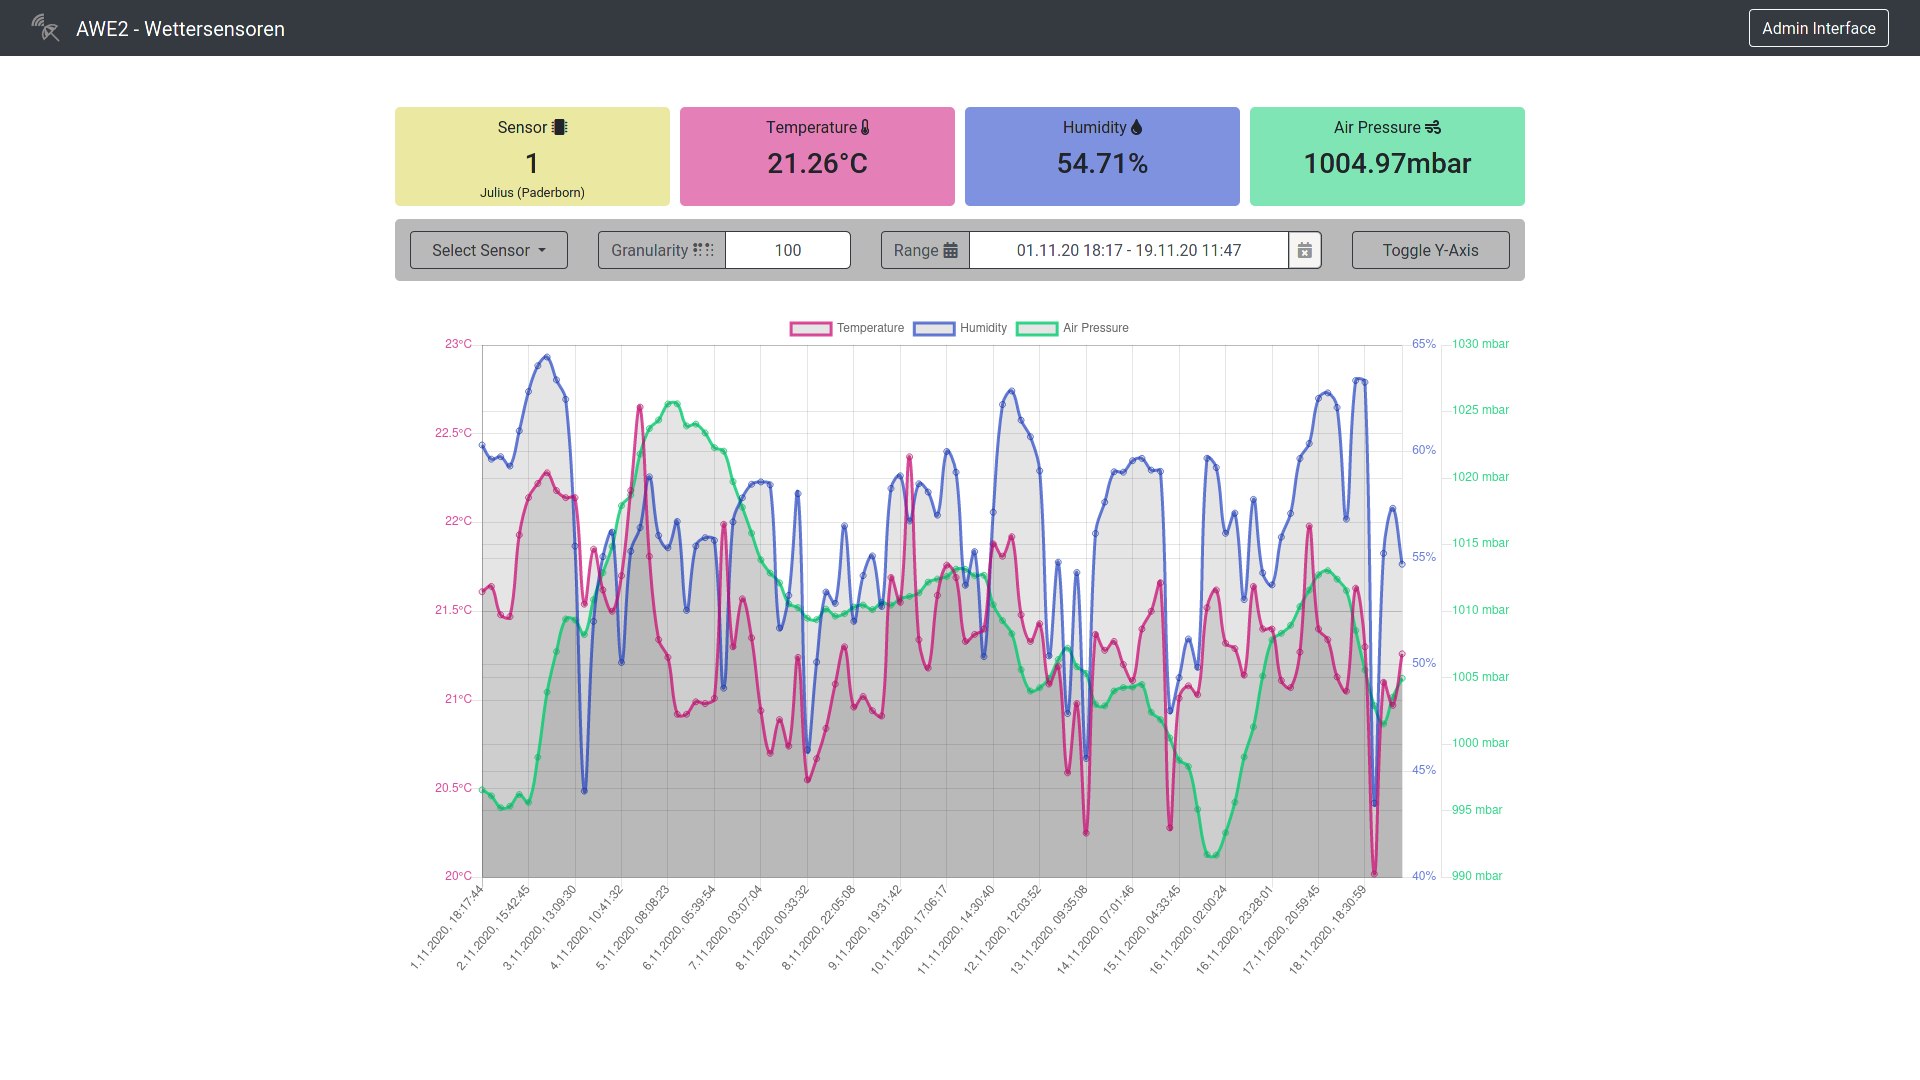
\includegraphics[width=1\textwidth]{img/gui-fertig.png}\\
        \source{Eigene Darstellung}
        \label{fig:finale-gui}
    \end{minipage}
\end{figure}

\pagebreak

\subanhang{Datumsauswahl}\label{datumsauswahl}

Die Datums- sowie Zeitauswahl beruht auf der Library \enquote{Date Range Picker}\footnote{\cite{daterangepicker.2020}}.
Diese ermöglicht eine einfache, ohne Anleitung verständliche, Auswahl des anzuzeigenden Zeitbereiches.
Auch hier wurden die Farben durch unsere Pastell-Farb-Palette angepasst.

\begin{figure}[h!!]
    \centering
    \begin{minipage}[t]{1\textwidth}
        \caption{Datumsauswahl Popup (finale GUI)}
        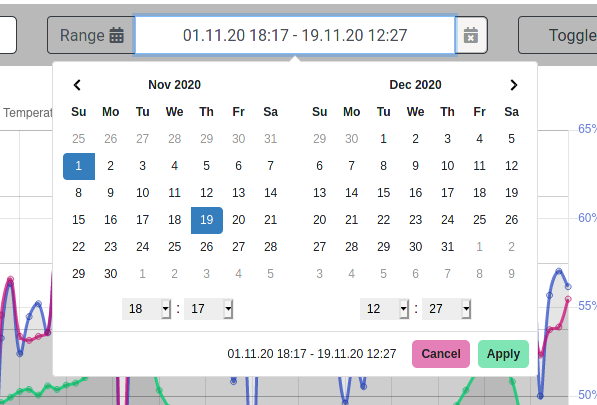
\includegraphics[width=1\textwidth]{img/datumsauswahl.png}\\
        \source{Eigene Darstellung}
        \label{fig:datumsauswahl}
    \end{minipage}
\end{figure}

\pagebreak

\subanhang{Admininterface}\label{admininterface}

Das Admininterface wurde einfach gehalten und greift wie die Hauptseite auf \enquote{Font-Awesome}\footnote{\cite{fontawesome}} für die Icons zurück.
Alle zur Verfügung stehenden Sensoren werden hier innerhalb einer Tabelle aufgelistet, der Standort des Sensors lässt sich einfach durch ein Inputfeld mit zugehörigem Button anpassen.
Bei erfolgreicher Eingabe wird eine positive Rückmeldung eingeblendet.
Diese findet sich beispielhaft in Anhang \ref{popup}.

\begin{figure}[h!!]
    \centering
    \begin{minipage}[t]{1\textwidth}
        \caption{Admininterface (finale GUI)}
        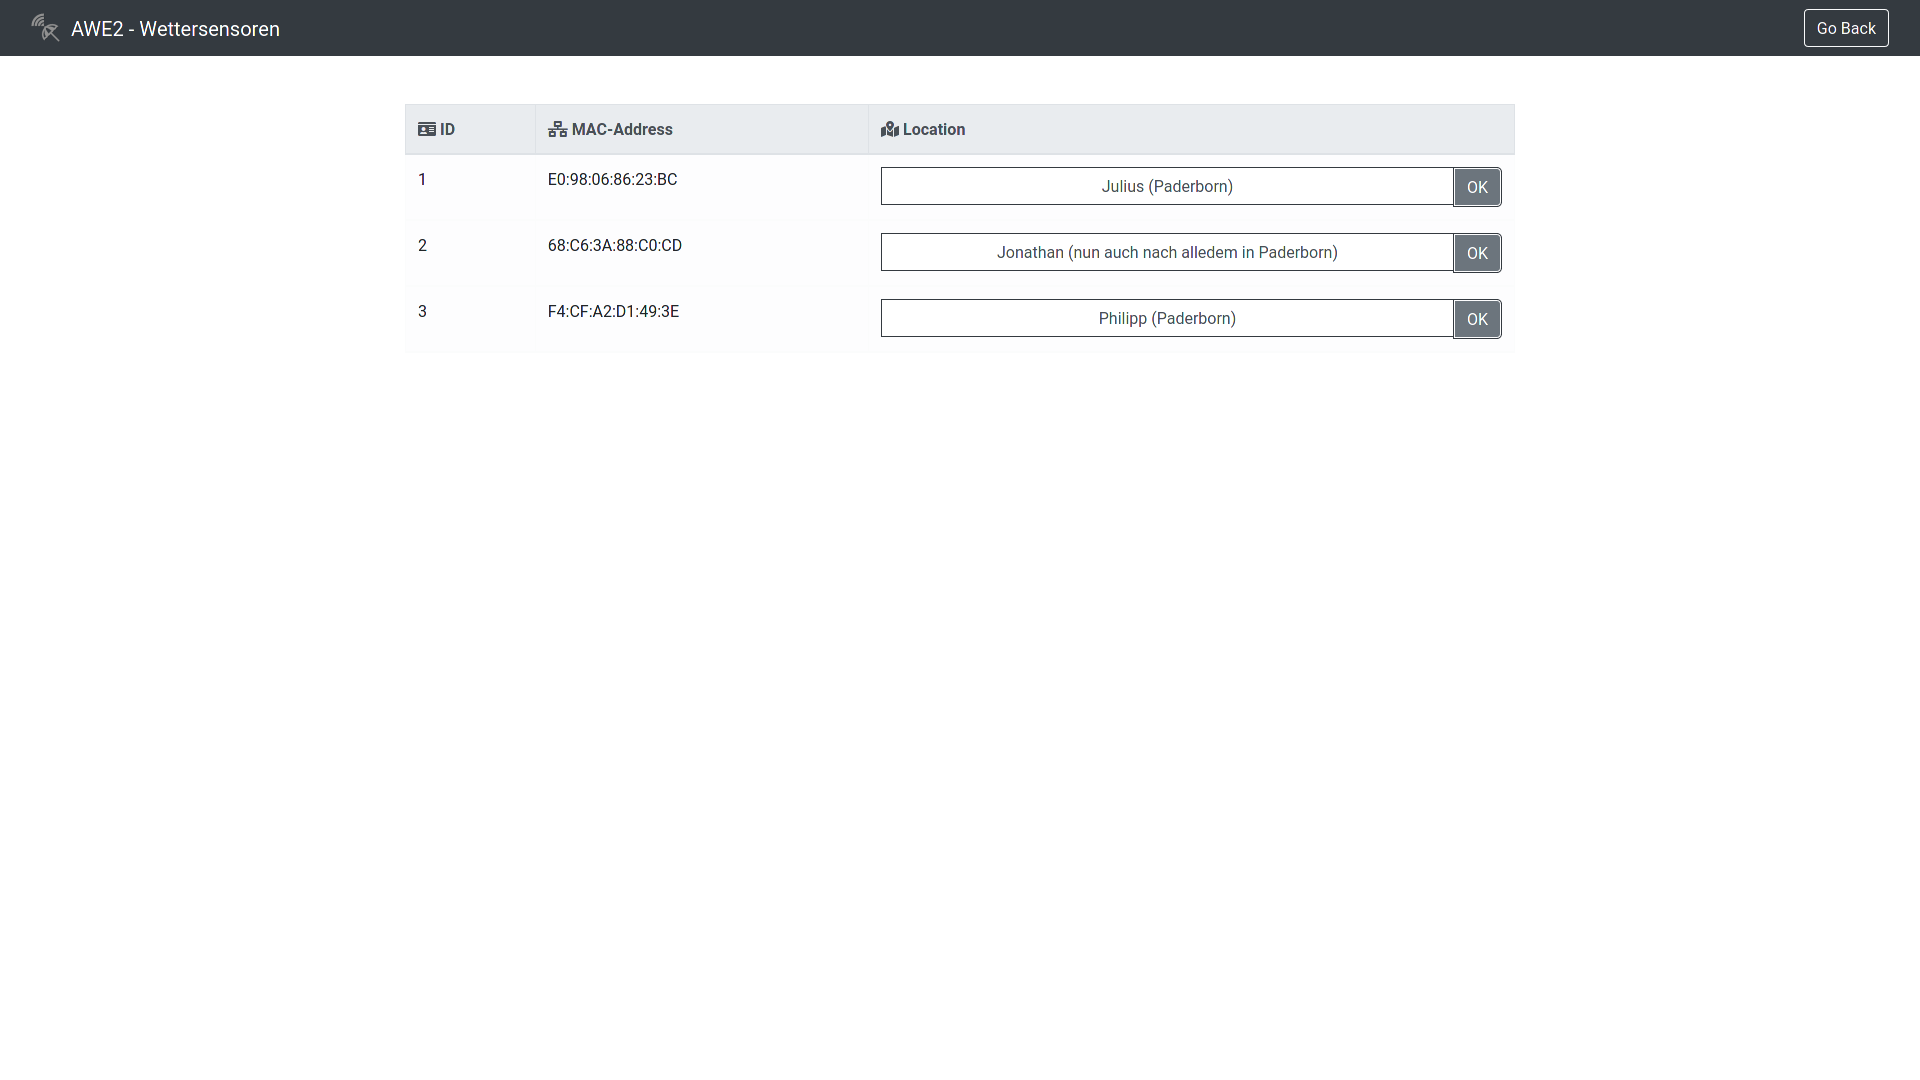
\includegraphics[width=1\textwidth]{img/admin.png}\\
        \source{Eigene Darstellung}
        \label{fig:admin}
    \end{minipage}
\end{figure}

\pagebreak

\subanhang{Informationsmeldungen}\label{popup}

Diese Einblendung wird zur Information des Nutzers angezeigt.
Neben dieser Darstellung welche nach erfolgreicher Änderung des Sensorstandortes eingeblendet wird, existiert eine \enquote{Error}-Version.
Diese ist in Rot gehalten und zeigt Fehler auf.

\begin{figure}[h!!]
	\centering
    \begin{minipage}[t]{1\textwidth}
        \caption{Informationsmeldung (finale GUI)}
        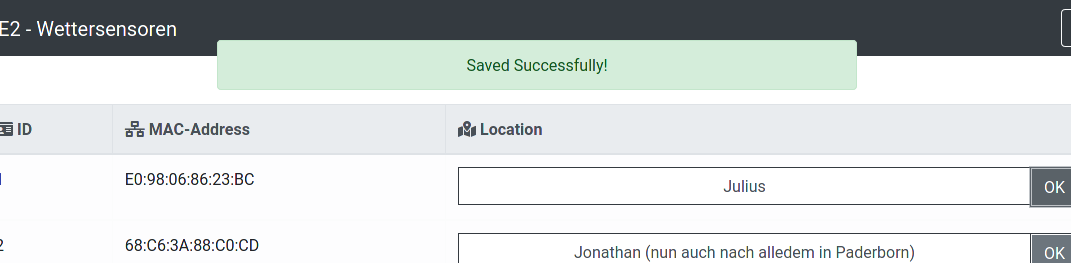
\includegraphics[width=1\textwidth]{img/popup.png}\\
        \source{Eigene Darstellung}
        \label{fig:datumsauswahl}
    \end{minipage}
\end{figure}

\pagebreak

\anhang{Soll-Ist-Vergleich}
\label{anh:sollist}

\begin{table}[H]
	\begin{tabular}{|l|l|l|}
		\hline
		\textbf{Anforderung}                                      & \textbf{Einstufung} & \textbf{Status}                  \\ \hline
		\begin{tabular}[c]{@{}l@{}}
			Es soll ein System zur dezentralen Erfassung von Daten \\ erstellt werden\\ Folgende Daten sollen erfasst werden: \\ Temperatur, Luftdruck, Luftfeuchtigkeit
		\end{tabular} & Muss & Erledigt \\ \hline
		Jedes Erfassungssystem ist ein Ort oder Raum fest verbunden & Muss & Erledigt \\ \hline
		\begin{tabular}[c]{@{}l@{}}
			Es gibt einen Server auf dem die Daten abgelegt werden\\ Server und Erfassungssystem müssen nicht im selben Intranet sein
		\end{tabular} & Muss & Erledigt \\ \hline
		\begin{tabular}[c]{@{}l@{}}
			Im Falle einer Kommunikationsunterbrechung werden die Daten \\ lokal gespeichert\\ Die Daten werden in diesem Fall übertragen sobald die Verbindung \\ wieder aufgebaut wird
		\end{tabular} & Kann & Erledigt \\ \hline
		\begin{tabular}[c]{@{}l@{}}
			Die Kommunikation soll mit minimalem Energieaufwand \\ durchgeführt werden
		\end{tabular} & Kann & Erledigt \\ \hline
		\begin{tabular}[c]{@{}l@{}}
			Die Erfassungsgeräte können auch über einen mobilen Hotspot \\ Daten an den Server senden
		\end{tabular}               & Kann               & Erledigt \\ \hline
		\begin{tabular}[c]{@{}l@{}}
			Die Daten sollen von einem beliebigen Ort mit Internetanschluss \\ abgerufen werden
		\end{tabular}               & Muss               & Erledigt \\ \hline
		Die Daten sollen grafisch dargestellt werden               & Muss               & Erledigt \\ \hline
		\begin{tabular}[c]{@{}l@{}}
			In der Darstellung der Daten können bestimmte Datentypen oder \\ einzelne Erfassungsysteme ausgewählt werden
		\end{tabular}               & Kann               & Erledigt \\ \hline
		Die Granularität der Daten ist variabel einstellbar               & Muss               & Erledigt \\ \hline
		\begin{tabular}[c]{@{}l@{}}
			Alle angeschlossenen Geräte sollen für einen Administrator \\ auf einer Plattform sichtbar sein
		\end{tabular}               & Muss               & Erledigt \\ \hline
		Mehrere Erfassungssystem pro Server sind möglich               & Muss               & Erledigt \\ \hline
		\begin{tabular}[c]{@{}l@{}}
			Ein Erfassungssystem kann mit verschiedenen \\ Servern kommunizieren
		\end{tabular}               & Kann               & Erledigt \\ \hline
		\begin{tabular}[c]{@{}l@{}}
			Es ist möglich zu sehen, wann der Sensor das letzte Mal \\ Daten gesendet hat
		\end{tabular}               & Bonus               & Erledigt \\ \hline
		Es ist möglich eine Wetterprognose anzuzeigen               & Bonus               & \begin{tabular}[c]{@{}l@{}}
																								Nicht\\ erledigt
		\end{tabular}               \\ \hline
	\end{tabular}
	\caption[Anforderungen]{Anforderungen (nach \cite{Wortmann.2020}, eigene Darstellung)}
\end{table}
\anhang{Projekt-Architektur}\label{anh:Projekt-Architektur}
\subanhang{Frontend}
\begin{figure}[H]
	\centering
	\begin{minipage}[t]{1\textwidth}
		\caption{Frontend-Ordnerstruktur}
		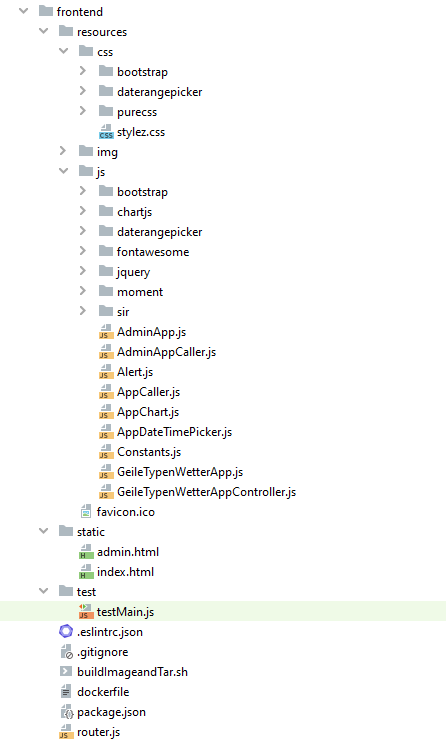
\includegraphics[width=0.5\textwidth]{img/dir_struc_frontend.png}\\
		\source{Eigene Darstellung}
		\label{fig:dir_struc_frontend}
	\end{minipage}
\end{figure}
\subanhang{Backend}
\begin{figure}[H]
	\centering
	\begin{minipage}[t]{1\textwidth}
		\caption{Backend-Ordnerstruktur}
		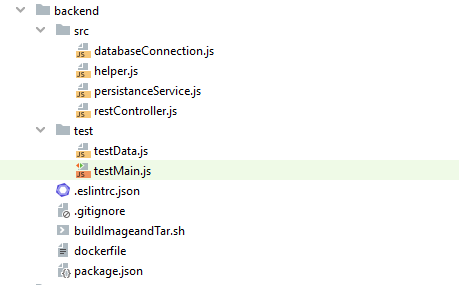
\includegraphics[width=0.5\textwidth]{img/dir_struc_backend.png}\\
		\source{Eigene Darstellung}
		\label{fig:dir_struc_backend}
	\end{minipage}
\end{figure}
\subanhang{NodeMCU}
\begin{figure}[H]
    \centering
    \begin{minipage}[t]{1\textwidth}
        \caption{NodeMCU-Ordnerstruktur}
        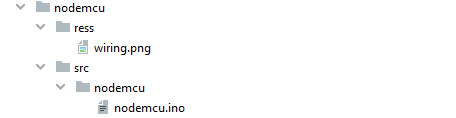
\includegraphics[width=0.5\textwidth]{img/dir_struc_nodemcu.png}\\
        \source{Eigene Darstellung}
        \label{fig:dir_struc_nodemcu}
    \end{minipage}
\end{figure}

\pagebreak

\anhang{Ausblick - Wetterprognose}\label{prognose}

In diesem Abschnitt findet sich eine Prototypische Implementierung die zu Psedudocode abgeändert wurde.
Für den spezifischen gewählten Sensor \textit{specificSensor} werden die \enquote{n}-letzten Datenpunkte benutzt um mit Hilfe der Funktion \textit{calculateTrends} eine Regressionsgerade über diese zu erzeugen. Hierzu werden zwei Hilfsfunktionen herangezogen. Die Funktion \textit{createDataPointTuplos} erzeugt aus den Sensordaten ()\textit{sensorData}) einen mehrdimensionalen Array welcher von der Library (hier beispielhaft anhand \textit{regressionLibrary}) zur Erzeugung der linearen Regressionsgeraden verwendet wird.
Des weiteren wird die Funktion \textit{getLowerBoundsGranularityOrSensordataLength} herangezogen um sicherzustellen dass keine \enquote{Out-of-Bounds}-Exceptions auftreten, indem der geringere Wert, anhand der Menge der vorhandenen Daten sowie den \enquote{n}-gewünschten Datenpunkten erzeugt wird.

\subanhang{Pseudocode Umsetzung}
\begin{figure}[bht]
    \begin{lstlisting}[caption=Pseudocode Regressionsgerade, label=list:regression]
		   calculateTrends(sensorData,specificSensor,granularity){
		 	let dataLength = this.
		 		getLowerBoundGranularityOrSensordataLength(sensorData, granularity)
		 	let trendData = this.
		 		createDataPointTuples(
		 			sensorData.timestamps.slice(-dataLength),
		 			sensorData.specificSensor.slice(-dataLength),
		 			dataLength
		 			);
		 	console.log(trendData);
		 	let trendSpecificSensor =
		 		regressionLibrary.linearRegression(trendData);
		 	console.log(trendSpecificSensor);
		 }

		 createDataPointTuples(timestamps,specificSensor, length){
		 	return Array.from({length: length}, (x, i) => {
		 		return [
		 			moment(timestamps[i],"DD.MM.YYYY, HH.mm.ss").unix(),
		 			specificSensor[i]
		 			];
		 	});
		 }

		 getLowerBoundGranularityOrSensordataLength(sensorData, granularity) {
		 	return sensorData.timestamps.length < granularity ?
		 		sensorData.timestamps.length : granularity;
		 }
    \end{lstlisting}
\end{figure}

\pagebreak

\subanhang{GUI Positionierung Konzeptuell}

In \cref{fig:posTrend} findet sich die Visualisierung der in \cref{list:regression} errechneten Daten.
Mit Hilfe der Steigung der Regressionsgerade wird das Icon eines Pfeils anhand von CSS im passenden Winkel rotiert.
Hierdurch ist direkt unter den aktuellen Werten der Trend in der Wertentwicklung sichtbar.
Idealerweise liesse sich dies noch durch einen Tooltip ergänzen, damit die Bedeutung des Pfeils für jeden intuitiv ersichtlich wird.

\begin{figure}[h!!]
    \centering
    \begin{minipage}[t]{1\textwidth}
        \caption{Positionierung Trend}
        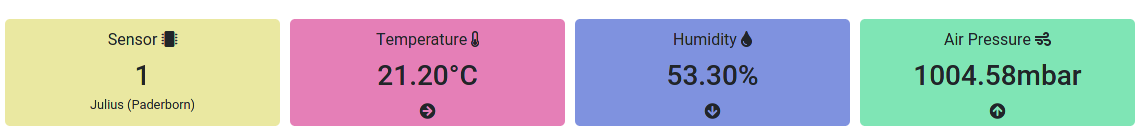
\includegraphics[width=1\textwidth]{img/konzept-trend.png}\\
        \source{Eigene Darstellung}
        \label{fig:posTrend}
    \end{minipage}
\end{figure}

\anhang{Ablaeufe}
\label{anh:ablaeufe}
\subanhang{Setup}
\begin{figure}[H]
    \centering
    \begin{minipage}[t]{1\textwidth}
        \caption{Zustandsdiagramm setup-Funktion}
        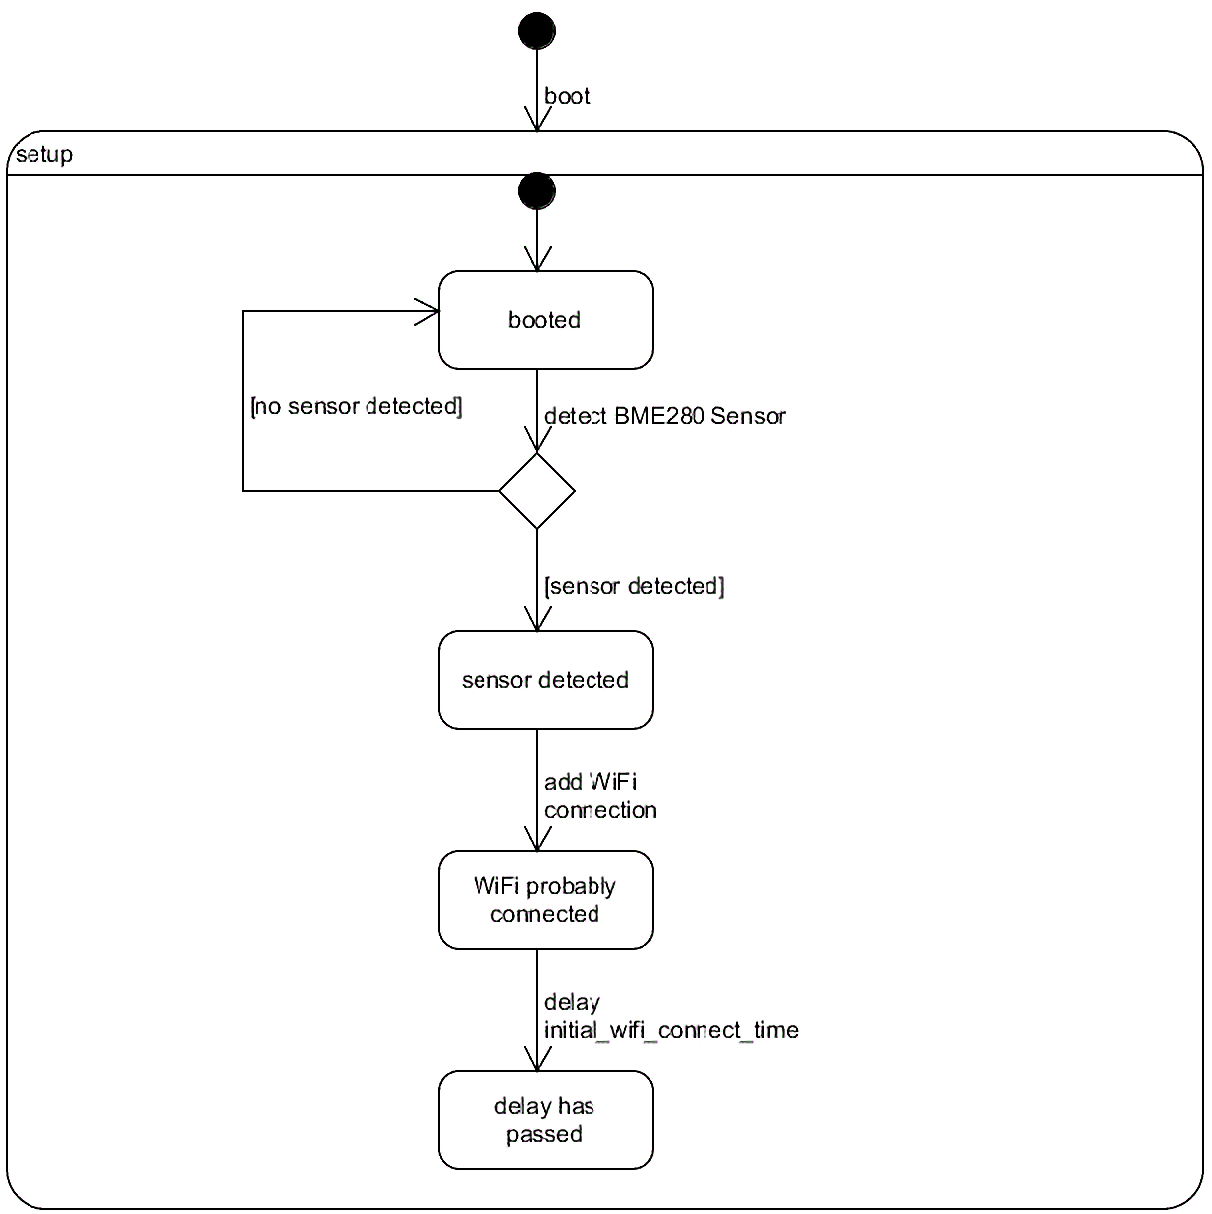
\includegraphics[width=1\textwidth]{img/zustandsdiagramm_nodemcu_setup.png}\\
        \source{Eigene Darstellung}
        \label{fig:zust_diag_nodemcu_setup}
    \end{minipage}
\end{figure}
\subanhang{Loop}
\begin{figure}[H]
    \centering
    \begin{minipage}[t]{1\textwidth}
        \caption{Zustandsdiagramm loop-Funktion}
        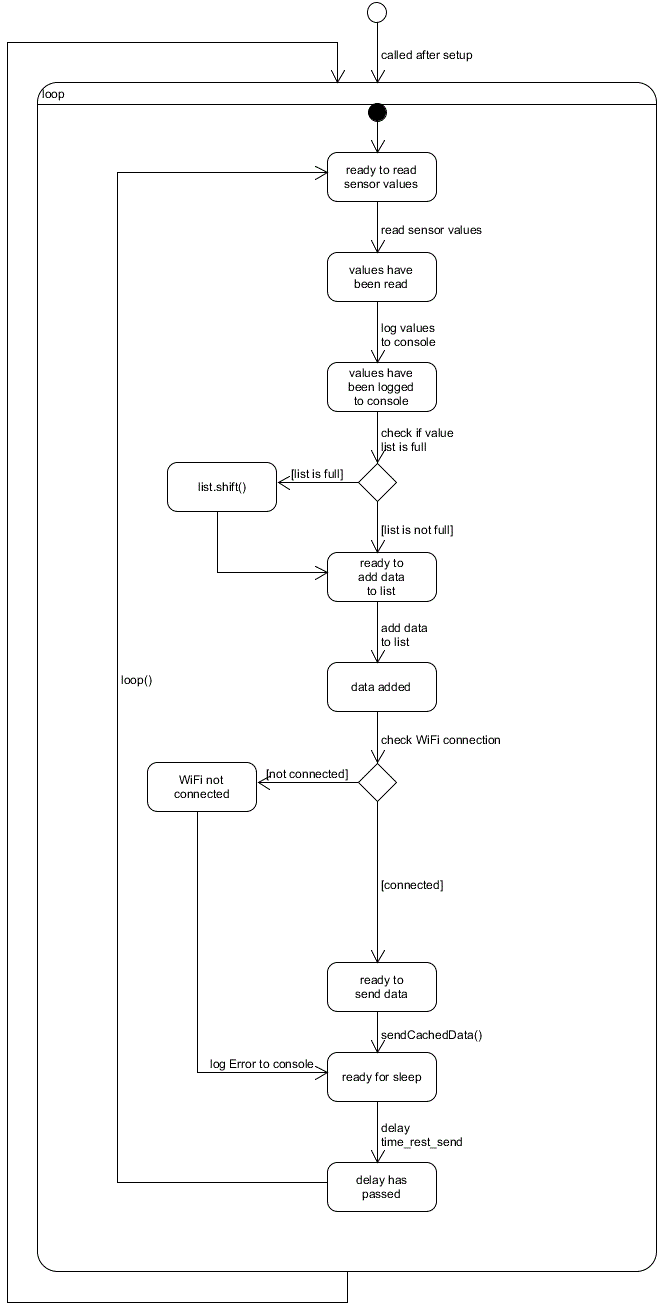
\includegraphics[width=0.60\textwidth]{img/zustandsdiagramm_nodemcu_loop.png}\\
        \source{Eigene Darstellung}
        \label{fig:zust_diag_nodemcu_loop}
    \end{minipage}
\end{figure}
\subanhang{SendCachedData}
\begin{figure}[H]
    \centering
    \begin{minipage}[t]{1\textwidth}
        \caption{Zustandsdiagramm sendCachedData-Funktion}
        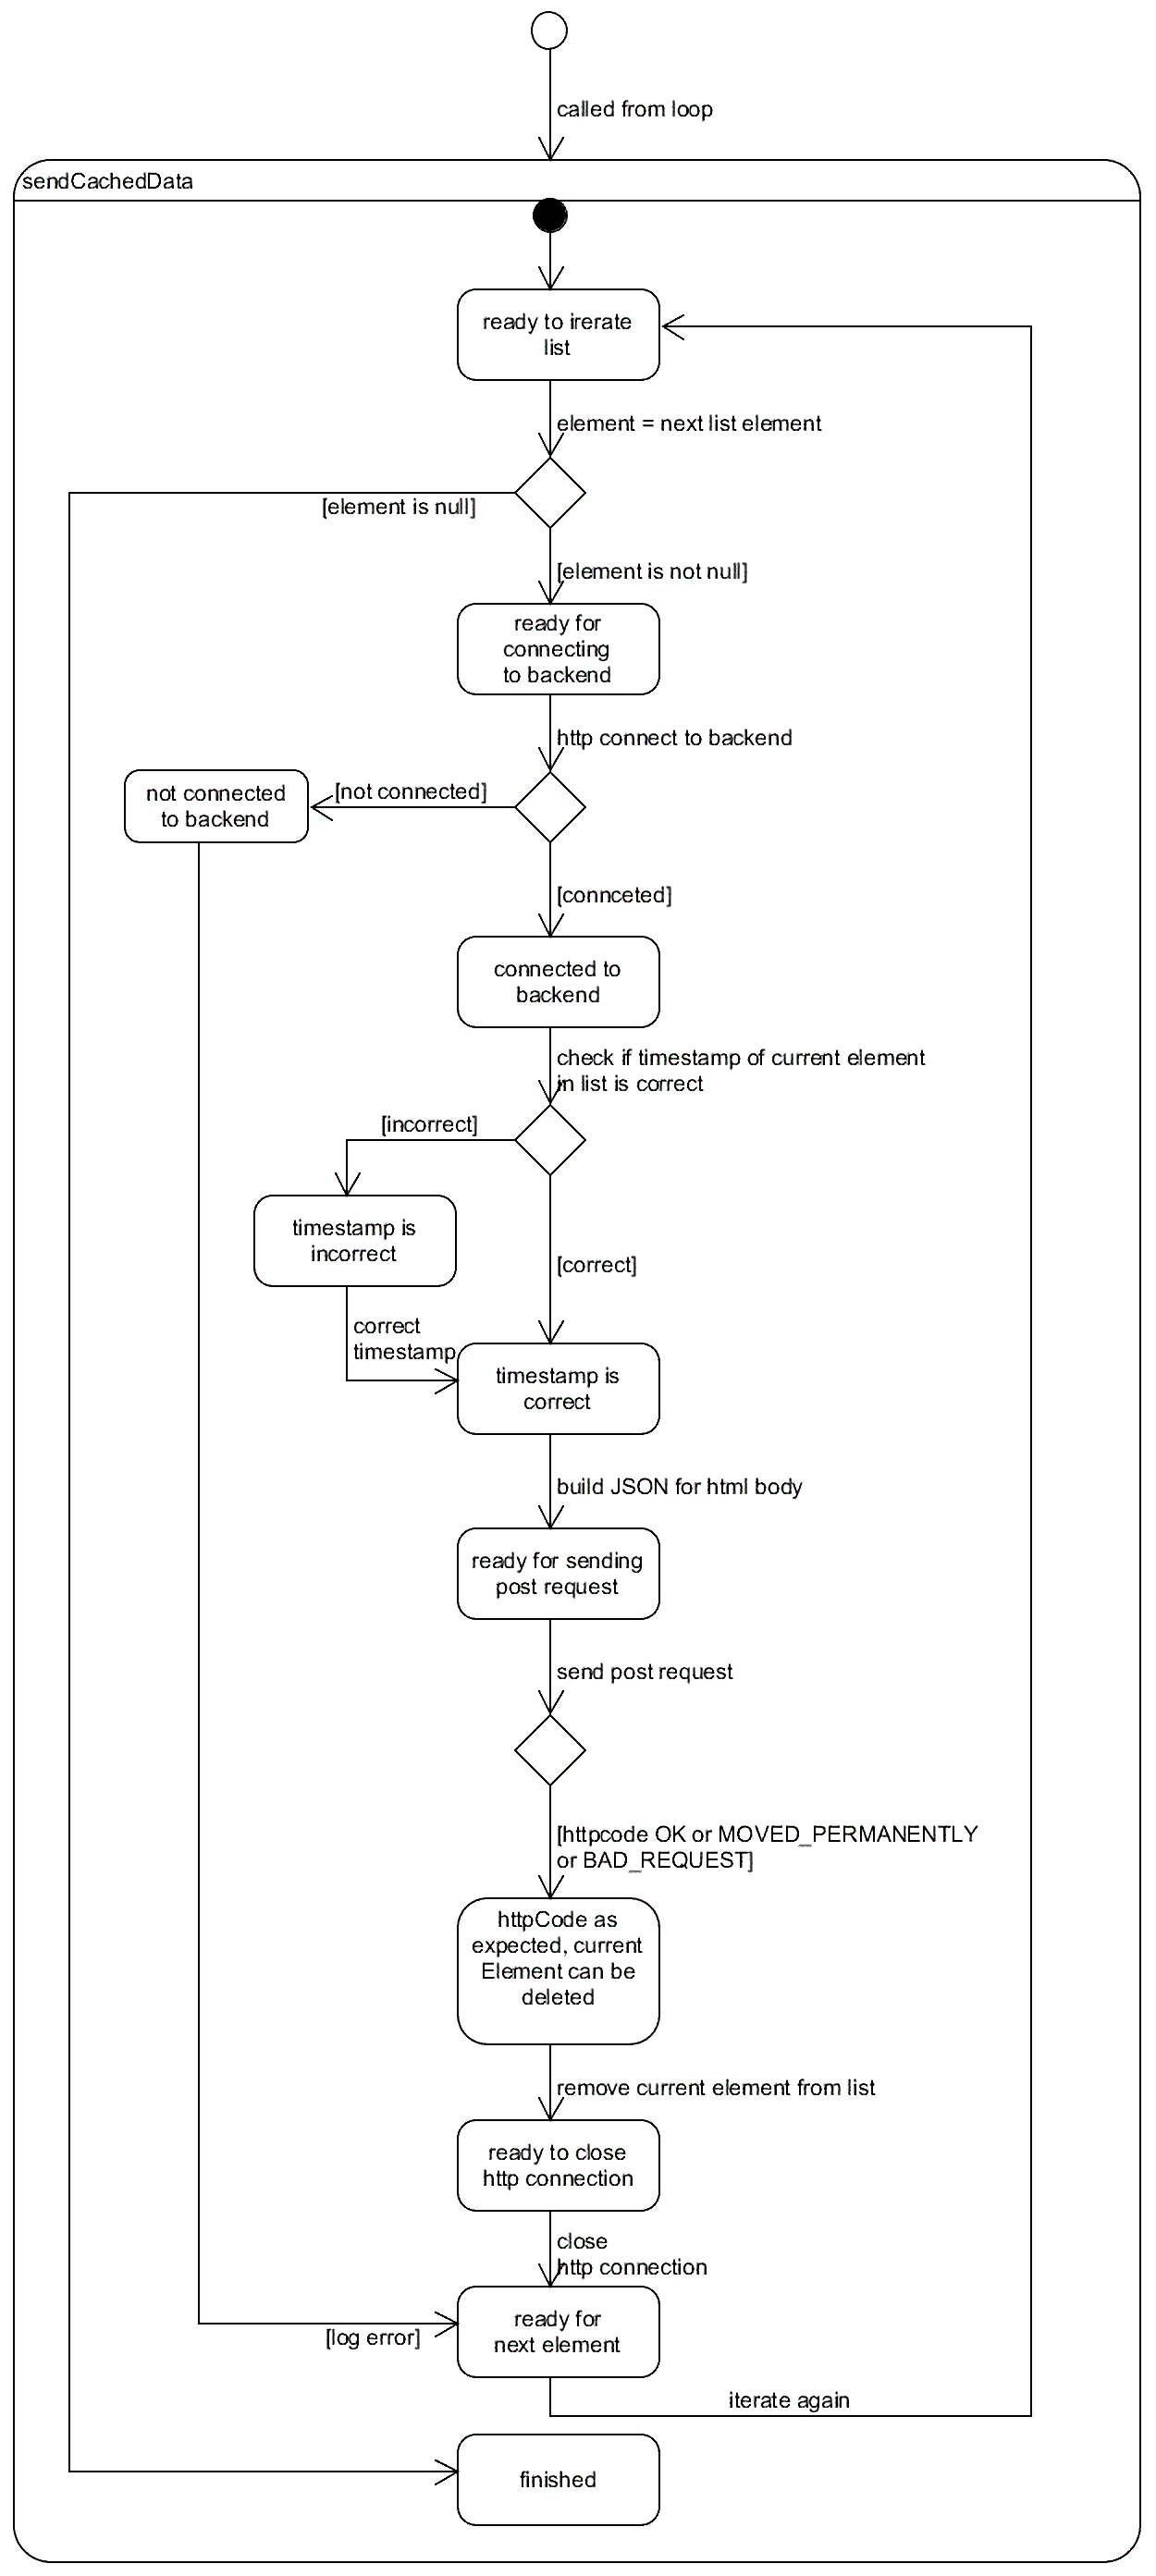
\includegraphics[width=0.55\textwidth]{img/zustandsdiagramm_nodemcu_sendCachedData.png}\\
        \source{Eigene Darstellung}
        \label{fig:zust_diag_nodemcu_send}
    \end{minipage}
\end{figure}